\section{Evaluation}
\label{sec:eval}

\subsection{Setup}
SemFault-250~\cite{yang2026semloc} has 250 single-function Python programs with one injected fault and about ten tests
each. We fix a stratified 50/200 dev/test split and group structurally similar programs into template clusters (4-gram
Jaccard on normalized code). Real bugs are the 31 youtube-dl bugs of BugsInPy~\cite{widyasari2020} whose environment
builds, whose triggering tests fail before and pass after the fix, and whose coverage can be measured; the target
function is the one containing a developer-changed line that a declared failing test executes. The renamed variant
replaces every program-defined identifier with an opaque name and blanks comments while preserving line numbers and
each test's outcome (199 test programs). The main model is Gemini~3.8 Flash; RQ3 adds GPT-6 luna, Claude Sonnet~5.5,
gpt-oss-120b and Gemini~3.5 Flash-Lite on a fixed 50-program subset. All models run at their provider-default reasoning
level; SemLoc runs at $T=\ConstTemperature$ as in the paper. Every LLM configuration is repeated three times; a run is
used only if it finished without unrecovered LLM errors. Differences are reported as $\Delta$ with \ConstCiLevel\% bootstrap CIs
that resample template clusters (\ConstBootstrapDraws{} draws), with per-program results averaged over repeats first.

\subsection{RQ1: Reproduction and evaluation audit}
All 13 published configurations reproduce exactly from the released logs. Table~\ref{tab:rq1} shows how scoring
matters: delta debugging scores \RqOneDdAuthorAllAccOne\% under the authors' scoring but \RqOneDdFairAllAccOne\% under
fair scoring, because it ranks no line; SBFL's Acc@5 rises from \RqOneSbflOchiaiAuthorAllAccFive\% to
\RqOneSbflOchiaiFairAllAccFive\%. SemLoc itself is stable under fair scoring, but removing the undocumented guess bonus
drops its Acc@1 from \RqOneSemlocClaudeTZeroEightFairAllAccOne\% to \RqOneSemlocClaudeTZeroEightNoPriorFairAllAccOne\%
(Claude) and from \RqOneSemlocGeminiTZeroEightFairAllAccOne\% to \RqOneSemlocGeminiTZeroEightNoPriorFairAllAccOne\%
(Gemini). In the released code the counterfactual step never changes a ranking (0 of 250 programs in all five
configurations with data); the gain the paper attributes to it matches the gap between two independent LLM runs. The
released BugsInPy runner reports the rank of the LLM's own guess rather than of the fixed lines, and its patch-and-restore
step leaves stale bytecode that can hide the bug in the next run; we fixed the latter in our driver. Repairing the
ground truth raises SemLoc's Acc@1 on our runs from \RqTwoOriginalAllSemlocAccOneMean\% to
\RqTwoRepairedAllSemlocAccOneMean\%; comparisons among SemLoc, the LLM baselines and CovGate keep their direction on both
ground truths.

\begin{table}[t]
\centering
\caption{Published configurations under the authors' and fair scoring (released logs, 250 programs)}
\label{tab:rq1}
\resizebox{\columnwidth}{!}{\begin{tabular}{lrrrrrr}
\toprule
 & \multicolumn{3}{c}{Author scoring} & \multicolumn{3}{c}{Fair scoring} \\
\cmidrule(lr){2-4}\cmidrule(lr){5-7}
Configuration (all 250 programs) & Acc@1 & Acc@3 & Acc@5 & Acc@1 & Acc@3 & Acc@5 \\
\midrule
SemLoc, Claude Sonnet 4.6, $T{=}0.8$ & 42.8 & 68.0 & 76.8 & 42.8 & 65.6 & 76.8 \\
SemLoc, Gemini 2.5 Pro, $T{=}0.8$ & 39.8 & 64.7 & 73.5 & 39.6 & 64.4 & 72.8 \\
SemLoc Claude $T{=}0.8$ without LLM-guess bonus & -- & -- & -- & 30.0 & 55.6 & 66.4 \\
SemLoc Gemini $T{=}0.8$ without LLM-guess bonus & -- & -- & -- & 27.2 & 55.6 & 64.0 \\
SemLoc w/o CF (separate run), Claude & 30.8 & 59.6 & 68.8 & -- & -- & -- \\
LLM direct, Claude & 35.2 & 41.2 & 41.2 & 35.2 & 41.2 & 41.2 \\
SBFL Ochiai & 6.4 & 13.2 & 30.4 & 4.0 & 16.0 & 48.0 \\
SBFL DStar (recomputed) & -- & -- & -- & 4.0 & 16.0 & 48.0 \\
Delta debugging & 38.0 & 38.0 & 38.0 & 0.0 & 0.0 & 0.0 \\
\bottomrule
\end{tabular}
}
\end{table}

\subsection{RQ2: Improvement and a simple baseline}
Table~\ref{tab:rq2} compares methods on the 200 test programs. LLM + coverage beats SemLoc on Acc@3 by
\RqTwoRepairedAllLlmCoverageDAccThree{} points [\RqTwoRepairedAllLlmCoverageDAccThreeLo,
\RqTwoRepairedAllLlmCoverageDAccThreeHi] and on Acc@1 by \RqTwoRepairedAllLlmCoverageDAccOne{}
[\RqTwoRepairedAllLlmCoverageDAccOneLo, \RqTwoRepairedAllLlmCoverageDAccOneHi]; it also wins on purely semantic faults,
where coverage alone cannot separate the fault (Acc@3 \RqTwoRepairedSemanticLlmCoverageAccThreeMean\% vs.\
\RqTwoRepairedSemanticSemlocAccThreeMean\%). Asking the LLM directly, without coverage, is not worse than SemLoc at Acc@1 ($\Delta$ \RqTwoRepairedAllLlmDirectDAccOne, CI includes zero) but loses
\RqTwoRepairedAllLlmDirectDAccThree{} points at Acc@3, so it is the coverage evidence, not the pipeline, that carries the
top-3 gain. Table~\ref{tab:label} splits the comparison by fault label. CovGate adds \RqTwoRepairedAllCovgateDAccThree{} points Acc@3 [\RqTwoRepairedAllCovgateDAccThreeLo,
\RqTwoRepairedAllCovgateDAccThreeHi] and leaves Acc@1 unchanged; its coverage gate alone gives most of that gain on the
repaired ground truth. Keeping the bonus only when execution supports the guess lowers Acc@1 by
\RqTwoRepairedAllGroundedPriorOnlyDAccOne{}, and counterfactual re-ranking lowers it by \RqTwoRepairedAllCfRerankDAccOne{}:
execution evidence does not separate right guesses from wrong ones.

\begin{table*}[t]
\centering
\caption{RQ2 on the test split (Gemini 3.8 Flash, three repeats; $\Delta$ vs.\ SemLoc with \ConstCiLevel\% cluster-bootstrap CI;
$r_{rb}$: matched-pairs rank-biserial on reciprocal rank)}
\label{tab:rq2}
\resizebox{0.9\textwidth}{!}{\begin{tabular}{lrrrrrr}
\toprule
Method & Acc@1 & Acc@3 & Acc@5 & $p_{\text{Acc@1}}$ & $p_{\text{Acc@3}}$ & $\delta_{\text{RR}}$ \\
\midrule
\multicolumn{7}{l}{\emph{Original ground truth, $n=200$, 2 repeats}} \\
SemLoc (as released) & 36.5{\scriptsize$\pm$0.7} & 59.0{\scriptsize$\pm$0.0} & 74.5{\scriptsize$\pm$0.0} & -- & -- & -- \\
\quad w/o LLM-guess bonus & 28.7{\scriptsize$\pm$1.8} & 56.2{\scriptsize$\pm$0.4} & 72.0{\scriptsize$\pm$0.7} & .050 & .070 & -0.08 \\
\quad + CF re-ranking & 34.5{\scriptsize$\pm$0.7} & 60.8{\scriptsize$\pm$0.4} & 76.8{\scriptsize$\pm$1.1} & .125 & .250 & -0.00 \\
CovGate (ours) & 36.5{\scriptsize$\pm$0.7} & 60.2{\scriptsize$\pm$0.4} & 74.5{\scriptsize$\pm$0.0} & 1.000 & .500 & +0.01 \\
CovGate + CF re-ranking & 34.5{\scriptsize$\pm$0.7} & 61.3{\scriptsize$\pm$0.4} & 76.8{\scriptsize$\pm$1.1} & .125 & .125 & +0.00 \\
LLM direct (1 prompt) & 40.0{\scriptsize$\pm$0.0} & 43.0{\scriptsize$\pm$0.7} & 43.2{\scriptsize$\pm$1.1} & .238 & $<$.001 & -0.21 \\
LLM + coverage (1 prompt, ours) & 40.5{\scriptsize$\pm$0.0} & 68.2{\scriptsize$\pm$0.4} & 70.5{\scriptsize$\pm$0.0} & .065 & .009 & +0.03 \\
SBFL Ochiai & 3.0{\scriptsize$\pm$0.0} & 15.5{\scriptsize$\pm$0.0} & 48.0{\scriptsize$\pm$0.0} & $<$.001 & $<$.001 & -0.47 \\
\midrule
\multicolumn{7}{l}{\emph{Execution-repaired ground truth, $n=190$, 2 repeats}} \\
SemLoc (as released) & 48.9{\scriptsize$\pm$0.7} & 70.3{\scriptsize$\pm$1.1} & 80.3{\scriptsize$\pm$1.9} & -- & -- & -- \\
\quad w/o LLM-guess bonus & 40.0{\scriptsize$\pm$2.2} & 65.8{\scriptsize$\pm$1.5} & 76.0{\scriptsize$\pm$2.6} & .050 & .012 & -0.11 \\
\quad + CF re-ranking & 46.6{\scriptsize$\pm$0.4} & 71.3{\scriptsize$\pm$0.4} & 81.0{\scriptsize$\pm$2.2} & .125 & 1.000 & -0.02 \\
CovGate (ours) & 48.9{\scriptsize$\pm$0.7} & 74.0{\scriptsize$\pm$1.1} & 80.0{\scriptsize$\pm$0.7} & 1.000 & .039 & +0.01 \\
CovGate + CF re-ranking & 46.6{\scriptsize$\pm$0.4} & 71.6{\scriptsize$\pm$1.5} & 80.8{\scriptsize$\pm$1.1} & .125 & .500 & -0.00 \\
LLM direct (1 prompt) & 53.2{\scriptsize$\pm$0.0} & 59.0{\scriptsize$\pm$0.7} & 59.2{\scriptsize$\pm$1.1} & .210 & .002 & -0.08 \\
LLM + coverage (1 prompt, ours) & 54.2{\scriptsize$\pm$0.7} & 86.8{\scriptsize$\pm$0.0} & 88.7{\scriptsize$\pm$0.4} & .039 & $<$.001 & +0.12 \\
SBFL Ochiai & 3.7{\scriptsize$\pm$0.0} & 17.9{\scriptsize$\pm$0.0} & 63.7{\scriptsize$\pm$0.0} & $<$.001 & $<$.001 & -0.53 \\
\bottomrule
\end{tabular}
}
\end{table*}

\begin{table}[t]
\centering
\caption{RQ2 by fault label (labels of the repaired ground truth)}
\label{tab:label}
\resizebox{\columnwidth}{!}{\begin{tabular}{lrrrrrrrrr}
\toprule
 & & \multicolumn{2}{c}{SBFL} & \multicolumn{2}{c}{SemLoc} & \multicolumn{2}{c}{CovGate} & \multicolumn{2}{c}{LLM + cov.} \\
\cmidrule(lr){3-4}\cmidrule(lr){5-6}\cmidrule(lr){7-8}\cmidrule(lr){9-10}
Fault label & $n$ & Acc@1 & Acc@3 & Acc@1 & Acc@3 & Acc@1 & Acc@3 & Acc@1 & Acc@3 \\
\midrule
Semantic & 162 & 1.8 & 17.3 & 54.7 & 77.6 & 54.7 & 81.1 & 60.1 & 91.8 \\
Coverage-revealed & 17 & 23.5 & 35.3 & 29.4 & 54.9 & 29.4 & 62.7 & 29.4 & 94.1 \\
Not executed & 11 & 0.0 & 0.0 & 0.0 & 3.0 & 0.0 & 0.0 & 0.0 & 0.0 \\
Executable (all but not executed) & 179 & 3.9 & 19.0 & 52.3 & 75.4 & 52.3 & 79.3 & 57.2 & 92.0 \\
\bottomrule
\end{tabular}
}
\end{table}

Table~\ref{tab:dec} answers the title. With both signals the game reproduces SemLoc exactly; at Acc@1 the guess
contributes \DecSemlocRepairedAllAccOnePhiGuess{} points [\DecSemlocRepairedAllAccOnePhiGuessCiClusterLo,
\DecSemlocRepairedAllAccOnePhiGuessCiClusterHi] and the spectrum \DecSemlocRepairedAllAccOnePhiSpectrum{}
[\DecSemlocRepairedAllAccOnePhiSpectrumCiClusterLo, \DecSemlocRepairedAllAccOnePhiSpectrumCiClusterHi]; at Acc@3 the
spectrum leads with \DecSemlocRepairedAllAccThreePhiSpectrum{} against \DecSemlocRepairedAllAccThreePhiGuess{}. On the
authors' own logs (Claude) the split is \PubSemlocClaudeTZeroEightSemlocOriginalAllAccOneFull{} =
\PubSemlocClaudeTZeroEightSemlocOriginalAllAccOnePhiGuess{} + \PubSemlocClaudeTZeroEightSemlocOriginalAllAccOnePhiSpectrum.

\begin{table}[t]
\centering
\caption{Grounded vs.\ guessed: Shapley split of SemLoc's accuracy (our runs, three repeats; template-cluster CIs)}
\label{tab:dec}
\resizebox{\columnwidth}{!}{\begin{tabular}{llrrrrr}
\toprule
Ground truth & Metric & Total & LLM guess & Semantic spectrum & Coverage & CF \\
\midrule
\multicolumn{7}{l}{\emph{SemLoc as released (guess + spectrum)}} \\
Original ($n=200$) & Acc@1 & 36.8 & 22.2{\scriptsize\,[16.5, 28.4]} & 14.6{\scriptsize\,[11.8, 17.5]} & -- & -- \\
Original ($n=200$) & Acc@3 & 60.3 & 19.8{\scriptsize\,[16.1, 23.8]} & 40.6{\scriptsize\,[35.6, 45.3]} & -- & -- \\
Repaired ($n=190$) & Acc@1 & 49.3 & 28.9{\scriptsize\,[22.0, 35.9]} & 20.3{\scriptsize\,[16.2, 24.7]} & -- & -- \\
Repaired ($n=190$) & Acc@3 & 71.2 & 26.8{\scriptsize\,[22.0, 31.9]} & 44.4{\scriptsize\,[39.3, 49.1]} & -- & -- \\
\midrule
\multicolumn{7}{l}{\emph{All signals (+ raw Ochiai, + CF re-ranking)}} \\
Original ($n=200$) & Acc@1 & 35.0 & 22.7{\scriptsize\,[17.4, 28.3]} & 12.5{\scriptsize\,[10.0, 15.2]} & -0.5{\scriptsize\,[-1.5, 0.6]} & 0.3{\scriptsize\,[-0.6, 1.1]} \\
Original ($n=200$) & Acc@3 & 59.0 & 17.6{\scriptsize\,[14.2, 21.4]} & 35.8{\scriptsize\,[31.6, 40.2]} & 4.6{\scriptsize\,[0.1, 9.0]} & 1.1{\scriptsize\,[0.5, 1.8]} \\
Repaired ($n=190$) & Acc@1 & 47.0 & 30.1{\scriptsize\,[23.6, 36.5]} & 17.5{\scriptsize\,[13.4, 21.8]} & -1.0{\scriptsize\,[-2.1, 0.2]} & 0.4{\scriptsize\,[-0.6, 1.4]} \\
Repaired ($n=190$) & Acc@3 & 76.0 & 24.4{\scriptsize\,[19.6, 29.4]} & 41.9{\scriptsize\,[37.2, 46.6]} & 8.7{\scriptsize\,[5.2, 12.4]} & 0.9{\scriptsize\,[0.3, 1.7]} \\
\bottomrule
\end{tabular}
}
\end{table}

\textbf{Cost.} SemLoc spends \CostSemlocTokensK k tokens per program, and its counterfactual step accounts for
\CostCfSharePct\% of its LLM calls; LLM + coverage spends \CostLlmCoverageTokensK k. Fig.~\ref{fig:pareto} places five
models on the same subset: for every model, LLM + coverage has higher Acc@3 at lower cost than SemLoc (per-model
differences have no CIs, and at Acc@1 GPT-6 luna does not improve).

\begin{figure}[t]
\centering
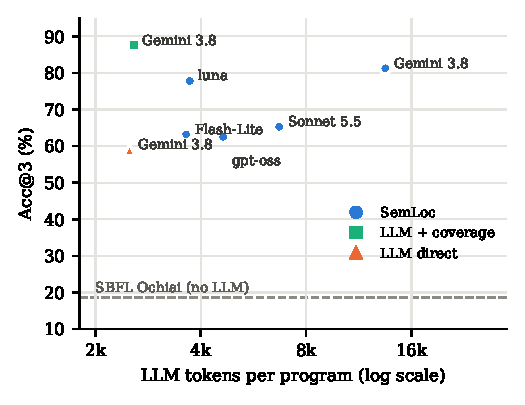
\includegraphics[width=\columnwidth]{../generated/pareto.pdf}
\caption{Cost vs.\ Acc@3 on the same 50-program subset (repaired ground truth); lines join the two methods of one model.}
\label{fig:pareto}
\end{figure}

\subsection{RQ3: Robustness}
\textbf{Real bugs.} On the 31 BugsInPy bugs (Table~\ref{tab:bip}), SemLoc's Acc@1 (\BipAllSemlocPriorAccOneMean\%)
equals that of the LLM's guess alone (\BipAllLlmGuessAccOneMean\%): every top-1 hit is the guess. The spectrum alone
reaches \BipAllSemlocSpectrumAccOneMean\%, close to SBFL (\BipAllSbflOchiaiAccOneMean\%). LLM + coverage points the same
way as on SemFault-250 (Acc@3 \BipAllLlmCoverageAccThreeMean\% vs.\ \BipAllSemlocPriorAccThreeMean\%), but with 31 bugs
the CI [\BipAllLlmCoverageDAccThreeLo, \BipAllLlmCoverageDAccThreeHi] includes zero.

\begin{table}[t]
\centering
\caption{RQ3a: 31 youtube-dl bugs (BugsInPy), three repeats}
\label{tab:bip}
\resizebox{\columnwidth}{!}{\begin{tabular}{lrrrrr}
\toprule
 & \multicolumn{3}{c}{All bugs ($n=31$)} & \multicolumn{2}{c}{Fault reached ($n=24$)} \\
\cmidrule(lr){2-4}\cmidrule(lr){5-6}
Method & Acc@1 & Acc@3 & Acc@5 & Acc@1 & Acc@3 \\
\midrule
SemLoc semantic spectrum only & 3.2{\scriptsize$\pm$0.0} & 23.7{\scriptsize$\pm$3.7} & 32.3{\scriptsize$\pm$3.2} & 4.2{\scriptsize$\pm$0.0} & 30.6{\scriptsize$\pm$4.8} \\
SemLoc (spectrum + LLM-guess bonus) & 44.1{\scriptsize$\pm$4.9} & 51.6{\scriptsize$\pm$5.6} & 53.8{\scriptsize$\pm$4.9} & 48.6{\scriptsize$\pm$6.4} & 58.3{\scriptsize$\pm$7.2} \\
LLM guess alone & 44.1{\scriptsize$\pm$4.9} & 44.1{\scriptsize$\pm$4.9} & 44.1{\scriptsize$\pm$4.9} & 48.6{\scriptsize$\pm$6.4} & 48.6{\scriptsize$\pm$6.4} \\
CovGate (ours) & 44.1{\scriptsize$\pm$4.9} & 52.7{\scriptsize$\pm$4.9} & 54.8{\scriptsize$\pm$5.6} & 48.6{\scriptsize$\pm$6.4} & 59.7{\scriptsize$\pm$6.4} \\
SBFL Ochiai & 6.5{\scriptsize$\pm$0.0} & 25.8{\scriptsize$\pm$0.0} & 25.8{\scriptsize$\pm$0.0} & 8.3{\scriptsize$\pm$0.0} & 33.3{\scriptsize$\pm$0.0} \\
SBFL DStar & 6.5{\scriptsize$\pm$0.0} & 25.8{\scriptsize$\pm$0.0} & 25.8{\scriptsize$\pm$0.0} & 8.3{\scriptsize$\pm$0.0} & 33.3{\scriptsize$\pm$0.0} \\
\midrule
Artifact's own metric (rank of the LLM guess) & 33.3{\scriptsize$\pm$1.9} & 38.7{\scriptsize$\pm$3.2} & 45.2{\scriptsize$\pm$3.2} & 31.9{\scriptsize$\pm$2.4} & 38.9{\scriptsize$\pm$6.4} \\
\bottomrule
\end{tabular}
}
\end{table}

\textbf{Renamed programs.} Pairing each program with its renamed copy (Table~\ref{tab:ren}), the guess barely moves (Acc@1
$\Delta$ \RenRepairedLlmGuessDAccOne{} [\RenRepairedLlmGuessDAccOneLo, \RenRepairedLlmGuessDAccOneHi]), so we see no sign
that the model guesses from memorized names. The constraint spectrum, however, needs meaningful names: without the bonus,
Acc@3 drops \RenRepairedSemlocNoPriorDAccThree{} points. LLM + coverage is unaffected (Acc@3 $\Delta$
\RenRepairedLlmCoverageDAccThree{} [\RenRepairedLlmCoverageDAccThreeLo, \RenRepairedLlmCoverageDAccThreeHi]).

\begin{table}[t]
\centering
\caption{RQ3b: original vs.\ identifier-renamed programs (repaired ground truth, three paired repeats)}
\label{tab:ren}
\resizebox{\columnwidth}{!}{\begin{tabular}{lrrrrrr}
\toprule
 & \multicolumn{3}{c}{Acc@1} & \multicolumn{3}{c}{Acc@3} \\
\cmidrule(lr){2-4}\cmidrule(lr){5-7}
Method & Original & Renamed & $p$ & Original & Renamed & $p$ \\
\midrule
SemLoc & 49.0{\scriptsize$\pm$0.8} & 46.6{\scriptsize$\pm$0.9} & .556 & 71.1{\scriptsize$\pm$1.9} & 63.0{\scriptsize$\pm$1.9} & .037 \\
\quad w/o LLM-guess bonus & 40.4{\scriptsize$\pm$2.0} & 32.5{\scriptsize$\pm$2.0} & .018 & 66.7{\scriptsize$\pm$2.1} & 51.8{\scriptsize$\pm$2.4} & $<$.001 \\
LLM guess alone & 49.0{\scriptsize$\pm$0.8} & 46.6{\scriptsize$\pm$0.9} & .556 & 49.0{\scriptsize$\pm$0.8} & 46.6{\scriptsize$\pm$0.9} & .556 \\
\bottomrule
\end{tabular}
}
\end{table}

\textbf{Model families.} Weaker models lean harder on the guess (Table~\ref{tab:fam}): without the bonus, Flash-Lite's
Acc@1 falls from \FamRepairedGeminiThreeFiveFlashLiteSemlocAccOneMean\% to
\FamRepairedGeminiThreeFiveFlashLiteSemlocNoPriorAccOneMean\% and gpt-oss-120b's from
\FamRepairedGptOssOneTwoZeroBSemlocAccOneMean\% to \FamRepairedGptOssOneTwoZeroBSemlocNoPriorAccOneMean\%, while Gemini~3.8
Flash barely changes.

\begin{table}[t]
\centering
\caption{RQ3c: five models on the same subset (repaired ground truth, three repeats)}
\label{tab:fam}
\resizebox{\columnwidth}{!}{\begin{tabular}{lrrrrrr}
\toprule
 & & \multicolumn{2}{c}{SemLoc} & \multicolumn{2}{c}{w/o LLM-guess bonus} & CovGate \\
\cmidrule(lr){3-4}\cmidrule(lr){5-6}\cmidrule(lr){7-7}
Model & Repeats & Acc@1 & Acc@3 & Acc@1 & Acc@3 & Acc@3 \\
\midrule
Gemini 3.8 Flash & 3 & 47.9{\scriptsize$\pm$2.1} & 80.6{\scriptsize$\pm$1.2} & 48.6{\scriptsize$\pm$4.3} & 77.8{\scriptsize$\pm$1.2} & 80.6{\scriptsize$\pm$2.4} \\
GPT-6 luna & 3 & 49.3{\scriptsize$\pm$2.4} & 77.8{\scriptsize$\pm$3.2} & 37.5{\scriptsize$\pm$5.5} & 67.4{\scriptsize$\pm$3.2} & 77.8{\scriptsize$\pm$1.2} \\
Claude Sonnet 5.5 & 3 & 39.6{\scriptsize$\pm$2.1} & 65.3{\scriptsize$\pm$1.2} & 34.7{\scriptsize$\pm$1.2} & 63.2{\scriptsize$\pm$1.2} & 65.3{\scriptsize$\pm$1.2} \\
gpt-oss-120b & 3 & 41.7{\scriptsize$\pm$5.5} & 62.5{\scriptsize$\pm$2.1} & 27.1{\scriptsize$\pm$7.2} & 53.5{\scriptsize$\pm$4.8} & 62.5{\scriptsize$\pm$2.1} \\
Gemini 3.5 Flash-Lite & 3 & 38.9{\scriptsize$\pm$3.2} & 63.2{\scriptsize$\pm$5.2} & 18.8{\scriptsize$\pm$2.1} & 50.7{\scriptsize$\pm$4.8} & 65.3{\scriptsize$\pm$1.2} \\
\bottomrule
\end{tabular}
}
\end{table}

\subsection{Failure analysis}
We categorize every test program automatically (Table~\ref{tab:fail}) and read a cluster-spread sample of up to four
failures per category, nineteen in total.

\begin{table}[t]
\centering
\caption{Per-program outcome categories (repaired ground truth, majority over three repeats); first match wins}
\label{tab:fail}
\scriptsize
\begin{tabularx}{\columnwidth}{@{}l>{\raggedright\arraybackslash}Xr@{}}
\toprule
Category & Definition & Programs \\
\midrule
gt\_suspect & unverified ground truth, every method misses top-3 & \FailGtSuspectN \\
guess\_right & the LLM's guess is a ground-truth line & \FailGuessRightN \\
prior\_hurts & spectrum ranks the fault first, the bonus lifts a wrong guess above it & \FailPriorHurtsN \\
rescued\_by\_spectrum & wrong guess, fault still in SemLoc's top-3 & \FailRescuedBySpectrumN \\
coverage\_only\_wins & SemLoc misses top-3, LLM + coverage hits it & \FailCoverageOnlyWinsN \\
all\_miss & everything else & \FailAllMissN \\
\bottomrule
\end{tabularx}
\end{table}
 The guess is right
for \FailGuessRightN{} of \FailProgramsN{} programs; the spectrum rescues \FailRescuedBySpectrumN{} wrong guesses into the
top three. Wrong guesses are rarely far off: across all repeats the guess hits the fault line \OffLlmGuessZeroCount{}
times, lands one line below it \OffLlmGuessOneCount{} times and one line above only \OffLlmGuessMinusOneCount{} times. In
\FailRelationHeaderBodyN{} of \FailWrongGuessN{} wrongly guessed programs, guess and ground truth are a compound-statement
header and the statement it guards, as in this program, where the injected fault is the \texttt{- 1}:
\begin{lstlisting}[numbers=left,firstnumber=63,escapeinside={(*}{*)}]
if cap is not None and counters[key] > cap: (*\textrm{\itshape\# ground truth}*)
    counters[key] = cap - 1                  (*\textrm{\itshape\# LLM's guess}*)
\end{lstlisting} Accepting either line raises SemLoc's Acc@1 from \TolSemlocAccOneExact\% to
\TolSemlocAccOneGuardStrict\% (strict) or \TolSemlocAccOneGuardOrBody\% (upper bound), and LLM + coverage's from
\TolLlmCoverageAccOneExact\% to \TolLlmCoverageAccOneGuardStrict\%--\TolLlmCoverageAccOneGuardOrBody\%; the ranking of
methods is unchanged. Reading the sample adds three more patterns: multi-line injected blocks where either line fixes the
bug, cause and symptom on one data-flow path, and fixes our oracle accepted that compensate rather than repair (e.g.,
\texttt{norm = norm() - 1} instead of fixing \texttt{max\_norm / (norm + 1)}). Most cases where the bonus ``hurts'' are of
the first two kinds: the guess is semantically right and one line off.
